\subsection{Savienojamība}
\begin{figure}[h]
    \label{att:desi_savienojamiba}
    \caption{DESI rādītāji}
    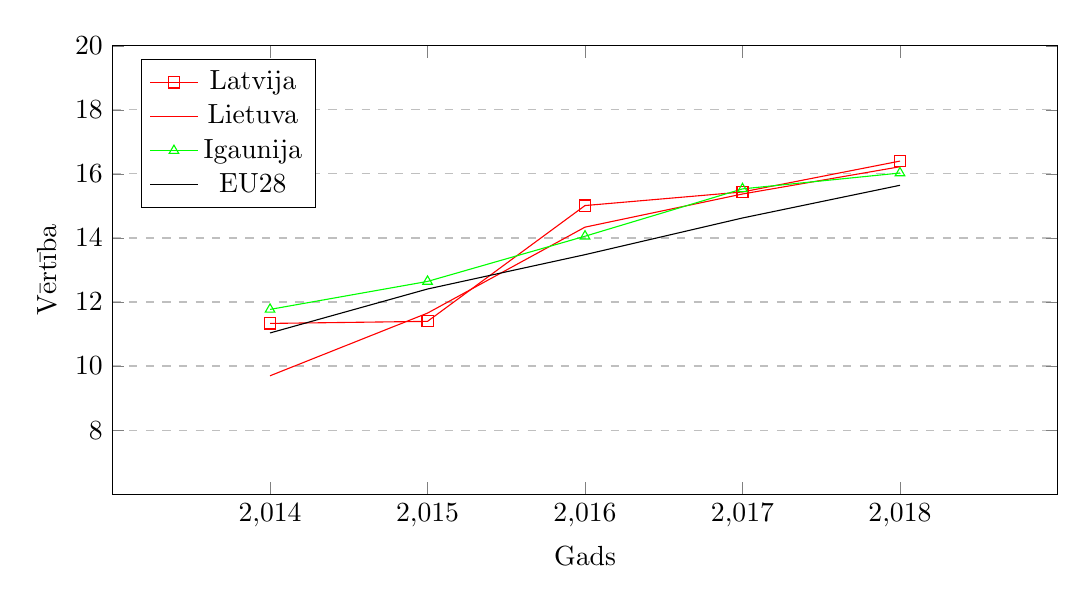
\begin{tikzpicture}
        \begin{axis}[
            x=2cm,
            xlabel={Gads},
            ylabel={Vērtība},
            xmin=2013, xmax=2019,
            ymin=6, ymax=20,
            xtick={2014,2015,2016,2017,2018},
            ytick={8,10,12,14,16,18,20},
            legend pos=north west,
            ymajorgrids=true,
            grid style=dashed,
        ]
        \addplot[
            color=red, 
            mark=square
            ]
            coordinates {
                (2014,11.3305)(2015,11.3951)(2016,15.0115)(2017,15.4357)(2018,16.4)
            };
        \addplot[
            color=red, 
            mark=circle
            ]
            coordinates {
                (2014,9.6959)(2015,11.6532)(2016,14.3374)(2017,15.3726)(2018,16.2237)
            };
        \addplot[
            color=green, 
            mark=triangle
            ]
            coordinates {
                (2014,11.7685)(2015,12.6421)(2016,14.0537)(2017,15.5321)(2018,16.0279)
            };
        \addplot[
            color=black, 
            mark=dot
            ]
            coordinates {
                (2014,11.0332)(2015,12.4053)(2016,13.478)(2017,14.6234)(2018,15.6445)
            };
        \legend{Latvija, Lietuva, Igaunija, EU28}
        \end{axis}
    \end{tikzpicture}
\end{figure}
\paragraph{}
2017. gadā Latvijai izdevās panākt diezgan lielu progresu kopējā savienojamības
aspektā, un tās izaugsmes temps līdzinājās ES vidējam. Attiecībā uz mājsaimniecību
fiksētās platjoslas pārklājumu valstī vērojama stagnācija – tā joprojām atpaliek no ES
vidējā rādītāja, ar 93\% mājsaimniecību pārklājumu Latvijai atrodoties 24. vietā.
Jāuzsver, ka gandrīz viss pārklājums nodrošina nākamās paaudzes piekļuvi (NPP)
(91\% mājsaimniecību) un pat ātrdarbīgo platjoslu (88\% mājsaimniecību), tādējādi
Latviju ierindojot starp vadošajām dalībvalstīm, kuru rādītāji krietni pārsniedz ES
vidējo. Arī 4G pārklājums Latvijā ir ļoti augsts (98\% mājsaimniecību). Ātrdarbīgās un
īpaši ātrdarbīgās platjoslas izmantošanas līmenis arī ir ievērojami augstāks par ES
vidējo: 42\% un 35\% mājokļu abonē ātrdarbīgas un īpaši ātrdarbīgas platjoslas
pakalpojumus, kas attiecīgi Eiropas Savienībā vidēji ir 33\% un 15,4\%. Tomēr,
neskatoties uz nelielu pieaugumu 2017. gadā, kopējā fiksētās platjoslas izmantošana
Latvijā vēl aizvien ir mazliet zem ES vidējā rādītāja. Šo tendenci zināmā mērā 
Digitālās ekonomikas un sabiedrības indekss 2018, ziņojums par Latviju. lpp. 4 no 11
kompensē daudz straujākais mobilās platjoslas pieslēgumu pieaugums, jo ir plašas
iespējas izvēlēties datu plānus par pieejamām cenām.
\paragraph{}
“Vidējās jūdzes projekts”, kas tika sākts 2012. gadā un kam piešķirts līdzfinansējums
no ES struktūrfondiem, lai lauku teritorijas savienotu ar valsts pamatinfrastruktūru,
tagad nonācis otrajā posmā. Plānots, ka otrā posma būvdarbi sāksies 2018. gada
pavasarī. Galvenokārt tie tiks veikti atlikušajās “baltajās” teritorijās (2014.–2015. gadā
apzināta 221 teritorija). Paredzēts, ka līdz 2020. gadam optiskie kabeļi tiks ierīkoti
2800 km garumā un izveidoti aptuveni 220 optiskā tīkla piekļuves punkti. Pēc tam
telesakaru operatoriem, izmantojot jauno tīklu, kas ļaus galalietotājiem piedāvāt
mazumtirdzniecības pakalpojumus, būs iespēja izveidot vietējās sakaru līnijas ar datu
pārraides ātrumu vismaz 30 Mbit/s (“pēdējā jūdze”). Tomēr šķiet, ka ne visur tiek
veiktas privātās investīcijas “pēdējās jūdzes” infrastruktūras izbūvē. Ir vajadzīgi
turpmāki centieni, piemēram, papildu valsts atbalsta shēmas un regulatīvi pasākumi,
lai novērtētu situāciju un piedāvātu risinājumus, kas attiecīgajos gadījumos ļautu
novērst ar “pēdējo jūdzi” saistīto plaisu. Iespēja mājās, pieslēdzoties no mobilajām
ierīcēm, izmantot mobilo operatoru nodrošinātos fiksētos sakaru pakalpojumus,
palīdz pārvarēt šo plaisu atsevišķos lauku apvidos, kur netiek veiktas investīcijas
“pēdējās jūdzes” savienojumos\cite{platjosla}
\paragraph{}
Optiskā tīkla izveidē un 4G pakalpojumu ieviešanā Latvija ir izvirzījusies starp
līderiem. Tomēr joprojām problemātiska ir digitālā plaisa, kas izveidojusies starp
pilsētu un laukiem. Lai to novērstu, praktisku labumu var sniegt nesen pieņemtie
noteikumi, ar kuriem tiek transponēta Platjoslas izmaksu samazināšanas direktīva.
Turklāt, lai nākotnē neatpaliktu no straujās savienojamības attīstības, visiem tirgus
dalībniekiem jābūt savlaicīgi pieejamiem piemērotiem spektra blokiem agrīnai 5G
tīkla izmēģināšanai un izvēršanai.
